%%
%% $Id$
%%
%% Copyright (c) 2007-2008 Christian Fehler
%% Copyright (c) 2007-2008 Benjamin Mies
%%


%### removes texlipse warnings


\myslide{Grammatiken}
{
    \begin{itemgroup}{}
	\item Eingabe von Grammatiken
		\begin{itemgroup}{}
		\item Reguläre Grammatiken
		\item Kontextfreie Grammatiken
		\end{itemgroup}
	\item Konvertierung von Grammatiken
	\end{itemgroup}
    
	\vfill{}
}

\myslide{Grammatiken}
{
  \begin{center}
    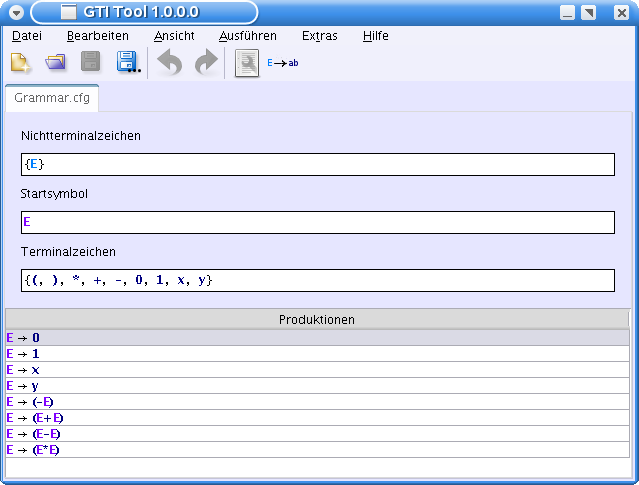
\includegraphics[height=14cm]{../images/cfg_example.png}
  \end{center} 
}

\myslide{Grammatiken - Reguläre Grammatik konvertieren}
{
    \begin{itemgroup}{}
	\item Es wird jede einzelene Produktion betrachtet
	\item Für das Nichtterminalzeichen auf der linken Seite wird ein Zustand
	angelegt.
	\item Besteht die rechte Seite aus einem einzelnen Terminalzeichen
  		\begin{itemgroup}{}
    	\item Einen Übergang zu einem akzeptierenden Zustand
    	\item Terminalzeichen als Produktionsmenge
    	\end{itemgroup}
	\item Besteht die rechte Seite aus einem Terminalzeichen und einem Nichtterminalzeichen
  		\begin{itemgroup}{}
    	\item Einen Übergang zu einem Zustand der das Nichterminalzeichen repräsentiert
		\item Terminalzeichen als Produktionsmenge
		 \end{itemgroup}
    \end{itemgroup}
	\vfill{}
}


\myslide{Grammatiken - Kontextfreie Grammatik konvertieren}
{
    \begin{itemgroup}{}
	\item Anlegen eines Startzustands
	\item Anlegen eines akzeptierenden Zustands
	\item Übergang von Startzustand in akzeptierenden Zustand bei dem das 
	Startsymbol auf den Keller gelegt wird
	\item Für jede Produktion ein Übergang vom akzeptierenden in akzeptierenden
	Zustand
		\begin{itemgroup}{}
    	\item Rechte Seite der Produktion vom Keller entfernen
    	\item Durch linke Seite der Produktion auf den Keller schreiben
    	\end{itemgroup}
	\item Für jedes Terminalzeichen ein Übergang vom akzeptierenden in akzeptierenden
	Zustand
		\begin{itemgroup}{}
    	\item Das Terminalzeichen wird vom Eingabeband gelesen und vom Keller
    	entfernt \end{itemgroup}
	\end{itemgroup}
  
	\vfill{}
}


%### removes texlipse warnings
